%
% The first command in your LaTeX source must be the \documentclass command.
\documentclass[sigconf]{acmart}
%
% defining the \BibTeX command - from Oren Patashnik's original BibTeX documentation.
\def\BibTeX{{\rm B\kern-.05em{\sc i\kern-.025em b}\kern-.08emT\kern-.1667em\lower.7ex\hbox{E}\kern-.125emX}}
    
% Rights management information. 
% This information is sent to you when you complete the rights form.
% These commands have SAMPLE values in them; it is your responsibility as an author to replace
% the commands and values with those provided to you when you complete the rights form.
%



%%%%%%%%%%%%%%5
\usepackage{lipsum}


\begin{document}

%
% The "title" command has an optional parameter, allowing the author to define a "short title" to be used in page headers.
\title{Collaborating Between Agile Teams}

%
% The "author" command and its associated commands are used to define the authors and their affiliations.
% Of note is the shared affiliation of the first two authors, and the "authornote" and "authornotemark" commands
% used to denote shared contribution to the research.
\author{Rakesh Mohan}
\author{Venkata Madhava Raju Akhil}
\email{amehlhase@asu.edu}

%
% The abstract is a short summary of the work to be presented in the article.
\begin{abstract}
A clear and well-documented \LaTeX\ document is presented as an article formatted for publication by ACM in 
a conference proceedings or journal publication. Based on the ``acmart'' document class, this article presents
and explains many of the common variations, as well as many of the formatting elements
an author may use in the preparation of the documentation of their work.
\end{abstract}


%
% Keywords. The author(s) should pick words that accurately describe the work being
% presented. Separate the keywords with commas.
\keywords{datasets, neural  networks, gaze detection, text tagging}

%
% A "teaser" image appears between the author and affiliation information and the body 
% of the document, and typically spans the page. 


%
% This command processes the author and affiliation and title information and builds
% the first part of the formatted document.
\maketitle


\section{Introduction}
The rise in the competition of in every industry means there is an increase in the uncertainty and volatility in every field which has resulted in an increase in the complexity of the software's. The increase in the complexity means the requirements of software is getting harder and harder to describe at the beginning of the project leading to a lot of ambiguity and incompleteness. That is why it so necessary to design for change rather execute the plan which also happens to be one of the manifesto of the agile methodology. Any new development these days are being managed by forming a small team with a team of developers having expertise in the required subject area. As more and more companies prefer agile methodology for project development it has led to situations when different agile teams have to work with each other to obtain a final end product. While this may sound easy for different teams to work together technically as they are implementing the same methodology there are so many hindrances that impedes the development process.


In [1] Alia Crocker, Rob Cross and Heidi K. Gardner discuss the issues faced by the organization Connected Commons which came upon a new innovative ground-breaking audio-visual technology which had potential to open up entirely new markets for the organization. The CEO considered it to be "pivot point" in organization growth and created a cross functional team to develop the application. But different teams assigned to this task struggled to develop the product as often they had problem in understanding the expertise or values of different function of other teams. At the same time fighting tooth and nail aggressively advocating for their own solution. Each team was surprised by the requirement of the external stakeholders thus showing how much the collaboration between the agile teams has hindered the progress of the product. This issue is not specific or unique to this organization alone it is quite the same situation whenever there is a necessity for different agile teams to work together.  

\begin{figure}
  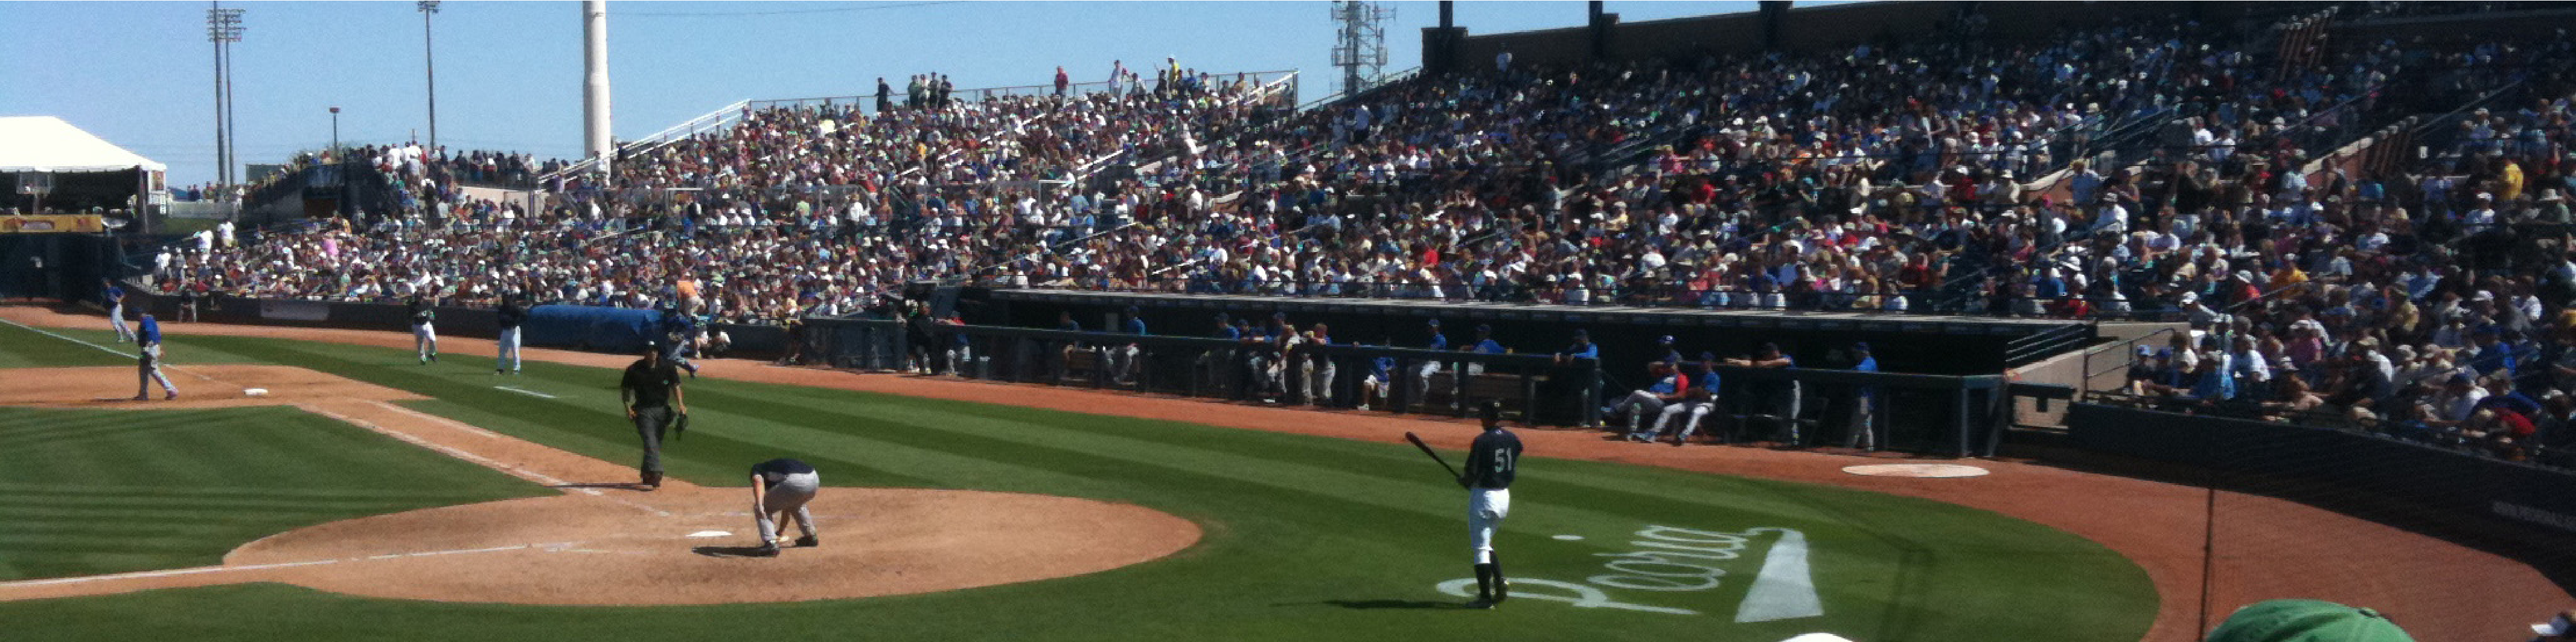
\includegraphics[width=0.5\textwidth]{sampleteaser}
  \caption{Seattle Mariners at Spring Training, 2010.}
  \Description{Enjoying the baseball game from the third-base seats. Ichiro Suzuki preparing to bat.}
  \label{fig:teaser}
\end{figure}

\section{TESTING}


\section{Verbatim}

\begin{verbatim}
  in here you can put any LaTeX commands and they will 
  not be evaluations \textbf{makes text bold}
\end{verbatim}

\section{Lists }

Bullet points:

\begin{itemize}
  \item first point
  \item second point
  \item third point
\end{itemize}

\noindent
Numbered list:
\begin{enumerate} %, [1)]
  \setcounter{enumi}{42}
  \item first point
  \item second point
  \item third point
\end{enumerate}


\noindent
Your own style:

\begin{itemize}
  \item[*] first point
  \item[] second point
  \item[=] third point
\end{itemize}


\section{Tables}
% \lipsum

Then you want a table \ref{tab:freq}. 

\begin{table}
  \caption{Frequency of Special Characters}
  \label{tab:freq}
  \begin{tabular}{lll}
    \toprule
    Non-English or Math   &   Frequency &   Comments\\
    \midrule
    \O                    & 1 in 1,000  & For Swedish names\\
    $\pi$                 & 1 in 5      & Common in math\\
    \$                    & 4 in 5      & Used in business\\
    $\Psi^2_1$            & 1 in 40,000 & Unexplained usage\\
  \bottomrule
\end{tabular}
\end{table}

To set a wider table, which takes up the whole width of the page's live area, use the environment \textbf{table*} to enclose the table's contents and the table caption.  
As with a single-column table, this wide table will ``float'' to a location deemed more desirable. Immediately following this sentence is the point at which Table~\ref{tab:commands} is included in the input file; again, it is instructive to compare the placement of the table here with the table in the printed output of this document.

\begin{table*}
  \caption{Some Typical Commands}
  \label{tab:commands}
  \begin{tabular}{ccl}
    \toprule
    Command &A Number & Comments\\
    \midrule
    \texttt{{\char'134}author} & 100& Author \\
    \texttt{{\char'134}table}& 300 & For tables\\
    \texttt{{\char'134}table*}& 400& For wider tables\\
    \bottomrule
  \end{tabular}
\end{table*}

\section{Math Equations}
You may want to display math equations in three distinct styles:
inline, numbered or non-numbered display.  Each of
the three are discussed in the next sections. 


\subsection{Inline (In-text) Equations}
A formula that appears in the running text is called an
inline or in-text formula.  It is produced by the
\textbf{math} environment, which can be
invoked with the usual \texttt{{\char'134}begin\,\ldots{\char'134}end}
construction or with the short form \texttt{\$\,\ldots\$}. You
can use any of the symbols and structures,
from $\alpha$ to $\omega$, available in
\LaTeX~\cite{Lamport:LaTeX}; this section will simply show a
few examples of in-text equations in context. Notice how
this equation:

\begin{math}
  \lim_{n\rightarrow \infty}x=0
\end{math},
set here in in-line math style, looks slightly different when
set in display style.  (See next section).

\subsection{Display Equations}
A numbered display equation---one set off by vertical space from the
text and centered horizontally---is produced by the \textbf{equation}
environment. An unnumbered display equation is produced by the
\textbf{displaymath} environment.

Again, in either environment, you can use any of the symbols
and structures available in \LaTeX\@; this section will just
give a couple of examples of display equations in context.
First, consider the equation, shown as an inline equation above:
\begin{equation}
  \lim_{n\rightarrow \infty}x=0
\end{equation}
Notice how it is formatted somewhat differently in
the \textbf{displaymath}

environment.  Now, we'll enter two unnumbered equations
\begin{displaymath}
  \sum_{i=0}^{\infty} x + 1
\end{displaymath}
\begin{equation*}
  \sum_{i=0}^{\infty} x + 1
\end{equation*}

and follow it with another numbered equation:
\begin{equation}
  \sum_{i=0}^{\infty}x_i=\int_{0}^{\pi+2} f
\end{equation}
just to demonstrate \LaTeX's able handling of numbering.


\section{Citations and Bibliographies}

The use of \BibTeX\ for the preparation and formatting of one's references is strongly recommended. Authors' names should be complete --- use full first names (``Donald E. Knuth'') not initials (``D. E. Knuth'') --- and the salient identifying features of a reference should be included: title, year, volume, number, pages, article DOI, etc. 

The bibliography is included in your source document with these two commands, placed just before the \verb|\end{document}| command:
\begin{verbatim}
  \bibliographystyle{ACM-Reference-Format}
  \bibliography{bibfile}
\end{verbatim}
where ``\verb|bibfile|'' is the name, without the ``\verb|.bib|'' suffix, of the \BibTeX\ file.

Citations and references are numbered by default. A small number of ACM publications have citations and references formatted in the ``author year'' style; for these exceptions, please include this command in the {\bf preamble} (before ``\verb|\begin{document}|'') of your \LaTeX\ source: 
\begin{verbatim}
  \citestyle{acmauthoryear}
\end{verbatim}

Some examples.  A paginated journal article \cite{Abril07}, an enumerated journal article \cite{Cohen07}, a reference to an entire issue \cite{JCohen96}, a monograph (whole book) \cite{Kosiur01}, a monograph/whole book in a series (see 2a in spec. document)
\cite{Harel79}, a divisible-book such as an anthology or compilation \cite{Editor00} followed by the same example, however we only output the series if the volume number is given \cite{Editor00a} (so Editor00a's series should NOT be present since it has no vol. no.),
a chapter in a divisible book \cite{Spector90}, a chapter in a divisible book in a series \cite{Douglass98}, a multi-volume work as book \cite{Knuth97}, an article in a proceedings (of a conference, symposium, workshop for example) (paginated proceedings article) \cite{Andler79}, a proceedings article with all possible elements \cite{Smith10}, an example of an enumerated proceedings article \cite{VanGundy07}, an informally published work \cite{Harel78}, a doctoral dissertation \cite{Clarkson85}, a master's thesis: \cite{anisi03}, an online document / world wide web resource \cite{Thornburg01, Ablamowicz07, Poker06}, a video game (Case 1) \cite{Obama08} and (Case 2) \cite{Novak03} and \cite{Lee05} and (Case 3) a patent \cite{JoeScientist001}, work accepted for publication \cite{rous08}, 'YYYYb'-test for prolific author \cite{SaeediMEJ10} and \cite{SaeediJETC10}. Other cites might contain 'duplicate' DOI and URLs (some SIAM articles) \cite{Kirschmer:2010:AEI:1958016.1958018}. Boris / Barbara Beeton: multi-volume works as books \cite{MR781536} and \cite{MR781537}. A couple of citations with DOIs: \cite{2004:ITE:1009386.1010128,Kirschmer:2010:AEI:1958016.1958018}. Online citations: \cite{TUGInstmem, Thornburg01, CTANacmart}.
%
% The next two lines define the bibliography style to be used, and the bibliography file.
\bibliographystyle{ACM-Reference-Format}%alpha
\bibliography{sample-base}

% 
% If your work has an appendix, this is the place to put it.
\appendix

\section{erer}

\end{document}
